\chapter{Resultados}

En este capitulo se presentan los resultados obtenidos de la ejecución del proyecto bajo ciertas condiciones representivas, con la intención de validar la funcionalidad y también de encontrar los puntos fuertes y las falencias del mismo.

\section{Configuración del Hardware}

\begin{center}
	\begin{longtable}{|l|p{4.75in}|} \hline
		\textbf{Feature} & \textbf{Description} \\ \hline
		FPGA & \begin{itemize}
			\item Cyclone II EP2C35F672C6 with EPCS16 16-Mbit serial configuration device.
			\end{itemize} \\ \hline
		I/O Interfaces &     \begin{itemize}
					\item Built-in USB-Blaster for FPGA configuration
    					\item Line In/Out, Microphone In (24-bit Audio CODEC)
   					\item Video Out (VGA 10-bit DAC)
   					\item Video In (NTSC/PAL/Multi-format)
   					\item RS232
    					\item Infrared port
   					\item PS/2 mouse or keyboard port
    					\item 10/100 Ethernet
   					\item USB 2.0 (type A and type B)
    					\item Expansion headers (two 40-pin headers)
				     \end{itemize} \\ \hline
		Memory & \begin{itemize}
					\item 8 MB SDRAM, 512 KB SRAM, 4 MB Flash
    					\item SD memory card slot
    			 \end{itemize} \\ \hline
		Displays & \begin{itemize}
					\item Eight 7-segment displays
    					\item 16 x 2 LCD display
    			 \end{itemize} \\ \hline
		Switches and LEDs & \begin{itemize}
					\item 18 toggle switches
    					\item 18 red LEDs
   					\item 9 green LEDs
   		 			\item Four debounced pushbutton switches
   				     \end{itemize} \\ \hline
		Clocks & \begin{itemize}
					\item 50 MHz clock
    					\item 27 MHz clock
   					\item External SMA clock input
   			 \end{itemize}	 \\ \hline
	\end{longtable} 
\end{center}

La FPGA incluida en la placa es una Cyclone II EP2C35 cuyas especificaciones son:

\begin{center}
	\begin{longtable}{|l|p{1.75in}|} \hline
		\textbf{Feature} & \textbf{Description} \\ \hline
		LEs & 33216 \\ \hline
		Total RAM bits & 483840 \\ \hline
		Embedded multipliers & 35 \\ \hline
		PLLs & 4 \\ \hline
		Maximum user I/O pins & 475 \\ \hline
	\end{longtable}
\end{center}

\subsection{Caso loopback}
\begin{figure}[h]
  \centering
	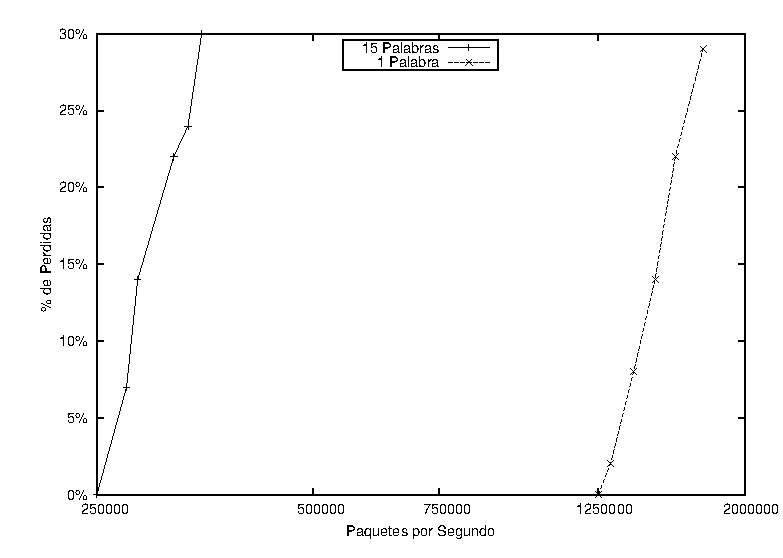
\includegraphics[width=0.70\textwidth]{5-resultados/graf/loop.eps}
  \caption{Caso Loopback para 1 y 15 palabras}
  \label{fig}
\end{figure}
En primera instancia nos ocupamos del caso loopback a los fines de encontrar los limites superiores de nuestro dise\~no.  En este caso, el software solo se limita a recibir los datos e inmediantemente después confirma el procesamiento y envía los resultados de regreso al hardware. Se realizan las pruebas correspondientes para las dos versiones de Uplink.
En el eje de las abscisas es posibles ver la cantidad de paquetes por segundo, el origen corresponde a la mayor velocidad a la que es posible transmitir sin perdidas. En las Ordenadas se puede observar la cantidad de paquetes perdidos en valores porcentuales, para obtener esta métrica se proceso una cantidad constante de paquetes, 9000, y luego se contrasto este valor con un contador global que el Generador estampa en la ultima palabra de cada paquete. Así se calculo la cantidad paquetes perdidos, sobre la cantidad total de paquetes generados. Este mismo sistema es el usado en todos los graficos posteriores.

\subsection{Caso Algoritmos unicamente}

Se estudiará la performance de los algoritmos aplicados, midiendo el retardo de lookup en funcion de la posición en la tabla de ruteo, se realizaran las pruebas de manera independiente al modulo extracto de cabeceras, para asi obtener una medida mas exacta del rendimiento.

\begin{figure}[h]
  \centering
	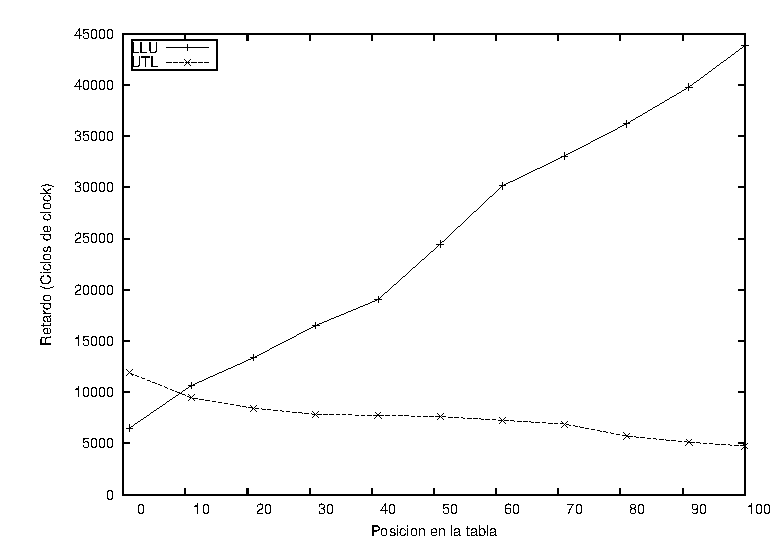
\includegraphics[width=0.8\textwidth]{5-resultados/graf/llu-utlsof.eps}
  \caption{Retardo de Busqueda LLU vs UTL}
  \label{fig}
\end{figure}

